%iffalse
\let\negmedspace\undefined
\let\negthickspace\undefined
\documentclass[journal,12pt,onecolumn]{IEEEtran}
\usepackage{cite}
\usepackage{amsmath,amssymb,amsfonts,amsthm}

\usepackage{graphicx}
\usepackage{textcomp}
\usepackage{xcolor}
\usepackage{txfonts}
\usepackage{listings}
\usepackage{enumitem}
\usepackage{mathtools}
\usepackage{gensymb}
\usepackage{comment}
\usepackage[breaklinks=true]{hyperref}
\usepackage{tkz-euclide} 
\usepackage{gvv}                                        
%\def\inputGnumericTable{}                                 
\usepackage[latin1]{inputenc}     
\usepackage{xparse}
\usepackage{color}                                            
\usepackage{array}                                            
\usepackage{longtable}                                       
\usepackage{calc}                                             
\usepackage{multirow}
\usepackage{multicol}
\usepackage{hhline}                                           
\usepackage{ifthen}                                           
\usepackage{lscape}
\usepackage{tabularx}
\usepackage{array}
\usepackage{float}
\newtheorem{theorem}{Theorem}[section]
\newtheorem{problem}{Problem}
\newtheorem{proposition}{Proposition}[section]
\newtheorem{lemma}{Lemma}[section]
\newtheorem{corollary}[theorem]{Corollary}
\newtheorem{example}{Example}[section]
\newtheorem{definition}[problem]{Definition}
\newcommand{\BEQA}{\begin{eqnarray}}
\newcommand{\EEQA}{\end{eqnarray}}
\newcommand{\define}{\stackrel{\triangle}{=}}
\theoremstyle{remark}
\newtheorem{rem}{Remark}
% Marks the beginning of the document

% Marks the beginning of the document
\begin{document}
\title{gate 1}
\author{AI25btech11022 - Narshitha}
\maketitle
\renewcommand{\thefigure}{\theenumi}
\renewcommand{\thetable}{\theenumi}
\begin {center}
\large \textbf{2007}\\
\large \textbf{CS:Computer science and Engineering}\\
\end{center}

\begin{center}
\textbf{Q.1-Q.20 carry one mark each}
\end{center}

\begin{enumerate}
\item    Consider the following two statements about the function $f(x)=|x|$ :
\newline
P: $f\brak{x}$ is continuous for all real values of $x$
\newline
 Q:$f\brak{x}$ is differentiable for all real values of $x$
 \newline
 Which of the following is \textbf{TRUE} ?

\begin{enumerate}
 

    \item  P is true and Q is false
    \item  P is false and Q is true
    \item Both P  and Q are true
    \item Both P and Q is false

\end{enumerate}
\hfill \textbf{(GATE EE 2025)}
\item    Let S be set of $n$ elements. The number of ordered pairs in the largest and the smallest equivalence relations on S are

\begin{enumerate}[label=(\Alph*)]
\begin{multicols}{4}
    \item $n$ and $n$
    \item $n^2$ and $n$
    \item $n^2$ and $0$
    \item $n$ and $1$
\end{multicols} 
\end{enumerate}
\hfill \textbf{(GATE EE 2025)}
    \item    What is the maximum number of different Boolean functions involving $n$ Boolean variables?
  
    \begin{enumerate}[label=(\Alph*)]
\begin{multicols}{4}
    \item $n^2$ 
    \item $2^{2^n}$
    \item $2^{2^n}$
    \item $2^{n^2}$ 
\end{multicols}
\end{enumerate}
\hfill \textbf{(GATE EE 2025)}


\item   Let G be the non planar graph with the minimum possible number of edges.Then G has

\begin{enumerate}

    \item $9$ edges and  $5$  vertices
    \item $9$ edges and  $6$  vertices
    \item $10$ edges and  $5$  vertices
    \item $10$ edges and  $6$  vertices

\end{enumerate}
\hfill \textbf{(GATE EE 2025)}

\item    Consider the DAG with $V=\cbrak{1,2,3,4,5,6}$ ,shown below.
\newline


    

\begin{figure}[h]
    \centering
    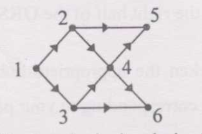
\includegraphics[width=0.2\columnwidth]{figs/fig1.png}
	\caption{ } 
    \label{fig1}
    

\end{figure}
   Which of the following is \textbf{NOT} a topological ordering?
   
\begin{enumerate}
\begin{multicols}{2}
    \item 1 2 3 4 5 6 
    \item 1 3 2 4 5 6 
    \item 1 3 2 4 6 5
    \item 3 2 4 1 6 5
\end{multicols}
\end{enumerate}
\hfill \textbf{(GATE EE 2025)}


\item  Which of the following problem is undecidale? 
\begin{enumerate}

    \item  Membership problem for CFGs
    \item Ambiguity problem for CFGs
    \item Finiteness problem for FSAs
    \item Equivalence problem for FSAs

\end{enumerate}
\hfill \textbf{(GATE EE 2025)}

 
\item   Which of the following is \textbf{TRUE}
\begin{enumerate}

    \item Every subset of a regular set is regular
    \item Every finite subset of a non-regular set is regular
    \item The union of two non-regular sets is not regular
    \item Infinite union of finite sets is regular

\end{enumerate}
\hfill \textbf{(GATE EE 2025)}
\item    How many 3-to-8 line decoders with an enable input are needed to  construct a 6-to-64 line decoder without using any other logic gates?
\begin{enumerate}
\begin{multicols}{4}
    \item 7 
    \item 8
    \item 9
    \item 10 
\end{multicols}
\end{enumerate}
\hfill \textbf{(GATE EE 2025)}
\item    Consider the following Boolean function of four variables:
\newline
 $f\brak{w,x,y,z}=\sum{1,3,4,6,9,11,12,14}$
 \newline
      the function is
\begin{enumerate}

    \item  independent of one variable
    \item  independent of two variables
    \item  independent of three variables
    \item  dependent of all the variables 

\end{enumerate}
\hfill \textbf{(GATE EE 2025)}
\item    Consider a $4$-way set associateve cache cosisting of $128$ lines with a line size of $64$ words. The CPU generates a 20-bit address of a word in main memory. The number of bits in the TAG,LINE and WORD fields are respectively:
\begin{enumerate}

\begin{multicols} {4}

   

    \item $ 9,6,5$
    \item $7,7,6$
    \item $7,5,8$
    \item $9,5,6$
\end{multicols}
\end{enumerate}
\hfill \textbf{(GATE EE 2025)}
\item     Consider a disk pack with $16$ surfaces ,$128 tracks per surface and $256 sectors per track. $512 $ bytes of data  are stored in a bit serial manner in a sector. The capacity of the disk pack and the number of bits required to specify a particular sector in the disk are respectively:
\begin{enumerate}
 

   \begin{multicols}{2}
       

    \item $256$ Mbyte,$19$Bytes    \item $256$  Mytes,$28$Bytes
    \item  $512$ Mytes,$20$Bytes \item  $64$ Mytes,$28$Bytes
    \end{multicols}

\end{enumerate}
\hfill \textbf{(GATE EE 2025)}
\item  The height of a binary tree is the maximum number of edges in any root to leaf path. The maximum number of nodes in a binary tree of height $h$ is:
\begin{enumerate}

\begin{multicols}{4} 

   

    \item $  2^h -1$
    \item $ 2^{h-1} -1$
    \item $2^{h+1} -1$
    \item $2^{h+1}$
    
\end{multicols}
\end{enumerate}
\hfill \textbf{(GATE EE 2025)}
\item    The maximum number of binary trees thst can be formed with three unlabeled nodes is:
\begin{enumerate}

\begin{multicols}{4} 

   

    \item $ 1$
    \item $5$
    \item $4$
    \item $3$
\end{multicols}
\end{enumerate}
\hfill \textbf{(GATE EE 2025)}
\item    Which of the following sorting algorithms has the lowest worst-case complexity?
\begin{enumerate}


\begin{multicols}{2}
   

    \item Merge sort 
    \item Bubble sort
    \item Quick sort 
    \item Selection sort 
\end{multicols}
\end{enumerate}
\hfill \textbf{(GATE EE 2025)}
  
\item    Consider the following segment of C-code:
\newline
     $int j,n;$
     \newline
    $  j=1;$
    \newline
    while $\brak{j<=n}$
    \newline
          $j=j*2;$
          \newline
The number of comparisions made in the execution of the loop for any $n>0$ is:
\begin{enumerate}
\begin{multicols}{4}
    \item $\lceil \log_{2} n \rceil +1$
    \item $n$
    \item  $\lceil \log_{2} n \rceil $
    \item $\lfloor \log_{2} n \rfloor +1 $
    \end{multicols}
    
\end{enumerate}
\hfill \textbf{(GATE EE 2025)}
    \item    Group $1$ contains some CPU scheduling algorithms and Group $2$ contains some applications. Match entries in Group $1$ to entries in Group $2$.
   
    
    
    \begin{tabular}{p{0.4\textwidth}p{0.5\textwidth}}


       \textbf{Group 1} &  \textbf{Group  2} \\ 
    P. Gang Scheduling &  1.  guarenteed Scheduling\\
   
    Q. Rate monotonic Scheduling &  2.  Real time Scheduling \\
     R.  Fair Share scheduling  &  3.Theard Scheduling \\
    \end{tabular}
\begin{enumerate}
    \begin{multicols}{2}
        \item P-3;Q-2;R-1
        \item P-1;Q-2;R-3
        \item P-2;Q-3;R-1
        \item P-1;Q-3;R-2
    \end{multicols}
\end{enumerate}
    \hfill \textbf{(GATE EE 2025)}
\item   Consider the following statements about user level threads and kernel level threads. Which one of the following statements is \textbf{FALSE}?
\begin{enumerate}
    \item  Context switch time  is longer for kernel level theards then for user level theards .
    \item User level threads do not need any hardware support.
    \item Related kernel level threads can be scheduled  on different processors in multi-processor  system 
    \item Blocking one kernel thread can block all other related threads
  \end{enumerate} 
 \hfill \textbf{(GATE EE 2025)}
  \item Which of the following is a top-down parser?
  \begin{enumerate}
      \item  Recurssive descent parser 
      \item Operator precedence parser.
      \item An LR \brak{k} parser.
      \item An LALR\brak{k} parser.
  \end{enumerate}
\hfill \textbf{(GATE EE 2025)}
\item In Ethernet when Manchester encoding is used,the bit rate is:
\begin{enumerate}
    \item Half the baud rate
\item Twice the baud rate
\item Same as baud rate
\item None of these
\end{enumerate}
\hfill \textbf{(GATE EE 2025)}
\item    Which one of the following uses UDP asthe transport protocol ?
\begin {enumerate}
\item HTTP
\item Telnet
\item DNS
\item SMTP
\end{enumerate}
\hfill \textbf{(GATE EE 2025)}

 
\begin{center}
    \textbf{Q.21 to Q.75 carry two marks each}
\end{center}
\item How many different non-isomorphic Abelian group of order $4$ are there?
\begin{enumerate}
\begin{multicols}{4}
    

    \item $2$
\item $3$
\item $4$
\item $5$
\end{multicols}
\end{enumerate}
\hfill \textbf{(GATE EE 2025)}
\item Let $Graph\brak{x}$ be a predicate which denotes that x is a graph. Let $connected\brak{x}$ be predicate which denotes that x is connected.which of the following first order logic sentences \textbf{DOES NOT} repressent the statement :"Not every graph  is connected" ?
\begin{enumerate}
    \item $\lnot\forall x \brak{Graph\brak{x}\implies Connected\brak{x}}$
    \item $\exists x \brak{Graph\brak{x}\land\lnot Connected\brak{x}}$
    \item $\lnot\forall x \brak{Graph\brak{x}\lor Connected\brak{x}}$
    \item $\forall x \brak{Graph\brak{x}\implies\lnot Connected\brak{x}}$
    
    \end{enumerate}
    \hfill \textbf{(GATE EE 2025)}
    \item Which of the following graphs has an Eulerian circuit?
    \begin{enumerate}
        \item Any k-regular graphs where k is an even number.
        \item a complete graph on $90$ vertices.
        \item The complement on a cycle on $25$ vertices.
        \item None of these
        \end{enumerate}
        \hfill \textbf{(GATE EE 2025)}
\item Suppose we uniformly and randomly select a permutation from the $20!$ permutations of $1,2,3,...,20.$ What is the probability that $2$ appears at an earlier position than any other even number  in selected permutation ?
\begin{enumerate}
    \item $\frac{1}{2}$   

    \item $\frac{1}{10}$

    \item $\frac{9!}{20!}$
  
    \item None of these
\end{enumerate}
\hfill \textbf{(GATE EE 2025)}
\item Let a $4 \times 4$ matrix with eigen values $-5,-2,1,4 $ Which of the following is the eigen value of
\begin{align}
    \myvec{A & I\\ I & A}
\end{align} 
,where I is the $4 \times 4$ identity matrix ?
\begin{enumerate}
    \item $-5$
    \item $-7$
    \item $2$
    \item $1$
\end{enumerate}
    
    \hfill \textbf{(GATE EE 2025)}
     
    \item consider the set $S=\cbrak{a,b,c,d}$.Consider the following four partitions $\pi_1,\pi_2,\pi_3,\pi_4$ on $S: \pi_1=\cbrak{\overline{abcd}},\pi_2=\cbrak{\overline{ab},\overline{cd}},\pi_3=\cbrak{\overline{abc},\overline{d}},\pi_4=\cbrak{\overline{a},\overline{b},\overline{c},\overline{d}}$ Let $\alpha$ br the partial  order set of partitions $S'=\cbrak{\pi_1,\pi_2,\pi_3,\pi_4}$ defined as follows :$\pi_i \alpha \pi_j$, if and only if $\pi_i$ refines $\pi_j$ .The poset diagram for $\brak{S',\alpha}$ is
   
        
         \begin{figure}[h]
            
            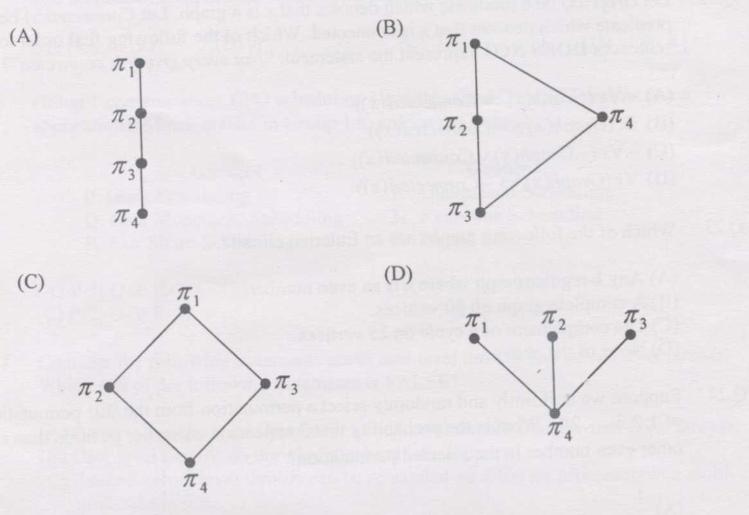
\includegraphics[width=0.9\linewidth]{figs/fig2.png}
		 \caption{ }
            \label{fig2}
            
        \end{figure}
        
 \hfill \textbf{(GATE EE 2025)}



    \item Consider the set of \brak{column} vectors defined  by  $X=\cbrak{x \in R^3| x_1 +x_2+x_3,where\quad x^r={\sbrak{x_1,x_2,x_3}}^T}$ Which of the following is \textbf{TRUE}?
    \begin{enumerate}
        \item $ \cbrak{{\sbrak{1,-1,0}}^T,{\sbrak{1,0,-1}}^T } $is basis for subspace X.
        \newline
        \item $ \cbrak{{\sbrak{1,-1,0}}^T,{\sbrak{1,0,-1}}^T } $ is a linerly independent set ,but it does not span X and therefore is not a basis  of X
        \item X is not a subspace of $R^3$
        \item None of these
    \end{enumerate}
    \hfill \textbf{(GATE EE 2025)}
    \item Consider the series $x_{n+1}=\frac{x_n}{2}+\frac{9}{8x_n},x_0=0.5$ obtained from the Newton-Raphson method The series converges to
    \begin{enumerate}
        \begin{multicols}{4}
        
   
        \item $1.5$
        \item $\sqrt{2}$
        \item $1.6$
        \item $1.4$
         \end{multicols}
    \end{enumerate}
    \hfill \textbf{(GATE EE 2025)}
    \item A minimum state deterministic finite automaton accepting the language 
    
        
 

      
  
      
\{
      
 
$L=\{w\mid w \in  \cbrak{0,1} ^ . \text{number of }  $0$\text{s and }$1$\text{s in w are divisible by } $3$ \text{ and } $5$\text{,respectively}$
 \}
      
  
  
    \begin{enumerate}
\begin{multicols}{4}
        
    
        \item 15 states 
        \item 11 states 
        \item 10 states
        \item 9 states 
        \end{multicols}
    \end{enumerate}
    \hfill \textbf{(GATE EE 2025)}
   
    \item The language $L= \cbrak{0^i 2 1^i| i\geq0}$ over the alphabet $\cbrak{0,1,2}$ is 
    \begin{enumerate}
        \item not recurssive 
        \item is recurssive and is a deterministic CFL
        \item is a regular language
        \item is not a deterministic CFL but a CFL
    \end{enumerate}
    \hfill \textbf{(GATE EE 2025)}
    \item Which of the following languages is regular?
    \begin{enumerate}
        \item $\cbrak{ww^R |w \in {\cbrak{0,1}}^+}$
        \item $\cbrak{ww^R x |x,w \in {\cbrak{0,1}}^+}$
        \item $\cbrak{wxw^R |x,w \in {\cbrak{0,1}}^+}$
        \item $\cbrak{xww^R |x,w \in {\cbrak{0,1}}^+}$
    \end{enumerate}
    \hfill \textbf{(GATE EE 2025)}
    \item Let $f\brak{w,x,y,z}=\sum (0,4,5,7,8,9,13,15)$ . Which of the following expressions are \textbf{NOT} equivalent to f ?
    \newline
    \brak{P} $ x'y'z' +w'xy' +wy'z+xz$
    \newline
    \brak{Q}$w'y'z'+ wx'y'+xz$
    \newline
    \brak{R} $w'y'z' +wx'y' +xyz +xy'z$
    \newline
    \brak{S}$x'y'z' +wx'y' +w'y$
\begin{enumerate}
    \item P only
    \item Q and S 
    \item R and S
    \item S only
\end{enumerate}    
\hfill \textbf{(GATE EE 2025)}
    \item Define the connective * for the Boolean variables X and Y. Considerthe following expresions P,Q and R.
    \newline 
    $P: X=Y*Z \quad  Q:Y=X*Z \quad R:X*Y*Z=1$
    \newline
    Which of the following is \textbf{TRUE} ?
    \begin{enumerate}
    \begin{multicols}{2}
        
  
        \item  Only P and Q are valid.
        \item  Only Q and R are valid.
        \item  Only P and R are valid.
        \item All P,Q,R are valid.
        \end{multicols}
        
    \end{enumerate}
    \hfill \textbf{(GATE EE 2025)}
    \item Suppose that only one multiplexer and one inverter are allowed to be used to implement any Boolean function of $n$ variables . What is the minimum size of the multiplexer needed?
    \begin{enumerate}
       \begin{multicols}{2}
           \item $2^n$ line to $1 $ line 
           \item $2^{n+1}$ line to $1$ line
           \item $2^{n-1}$ line to $1$ line
           \item $2^{n-2}$ line to $1$ line 
 \end{multicols}
    \end{enumerate}
    \hfill \textbf{(GATE EE 2025)}
     
    \item In a look-ahead carry generator, the carry generate function $ G_i$ and the carry propagate function $P_i$ for inputs $A_i$ and $B_i$ are given by :
    \newline 
    The expressions for the sum bit $S_i$ and the carry bit $C_{i+1}$ of thelook-ahead carry adder are given by :
    \newline 
    $S_i=P_i \oplus C_i$ and $C_{i+1}= G_i +P_i C_i$ where $C_0$ is the input carry.
    \newline 
    Consider a two-level logic implementation  of the look-ahead carry generator . Assume that all $P_i$ and $G_i$ are available for the carry generate circuit and that the AND and OR gates can have any number of inputs. The number of AND and OR gates  needed to implement the look-ahead carry generator  for a $4$-bit adder with $S_3,S_2,S_1,S_0$ and $C_4$ as its outputs are respectively:
    \begin{enumerate}
        \begin{multicols}{4}
        \item $6,3$
        \item $10,4$
        \item $6,4$
        \item $10,5$
        
            
        \end{multicols}
    \end{enumerate}
    \hfill \textbf{(GATE EE 2025)}
    \item The control signal functions of a $4$-bit binary counter are given below \brak{where X is "don't care "}:
    \newline
         \begin{tabular}{|c|c|c|c|c|}
         
        \hline 
      Clear & Clock & Load & Count & Function \\ \hline 
      1 & X & X & X & Clear to $0$ \\ \hline
      0 & X & 0 & 0 & No change \\ \hline
      0 & $\uparrow$ & 1 & X & Load input \\ \hline
      0 & $\uparrow$ & 1 & 1 & Count next \\ \hline
          
             
        \end{tabular}
 
     
  
       
       
    
        The counter is connected as follows:
       
            \begin{figure}[h]
                \centering
                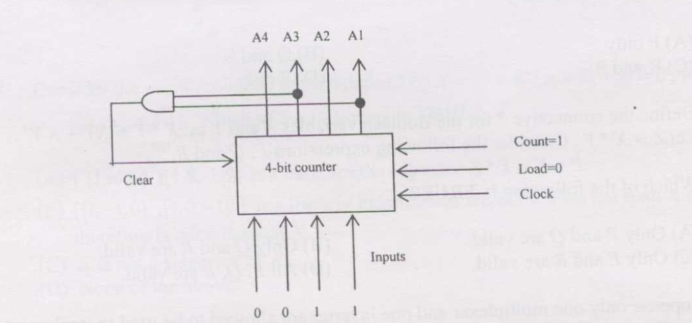
\includegraphics[width=0.9\linewidth]{figs/fig3.png}
                \caption{ }
                \label{fig3}
            \end{figure} 

            
          Assume that the counter and gate delays are negligible. If the counter starts at $0$ ,then it cycles through the following sequence :
            \begin{enumerate}
               \begin{multicols}{2}
               \item $0,3,4$
               \item $0,3,4,5$
               \item $0,1,2,3,4$
               \item $0,1,2,3,4,5$
                   
               \end{multicols} 
            \end{enumerate}
           \hfill \textbf{(GATE EE 2025)}
             
            \item Consider a pipelined processor with the following four stages :
            \newline
            IF: Instruction Fetch 
            \newline
            ID: Instruction Decode and Operand Fetch 
            \newline 
            EX : Execute
            \newline 
            WB : Write Back
            \newline
            The IF,ID and WB stages take one clock cycle each to complete the operation. The number of clock cycles  for the EX stage depends on the instruction. The ADD and SUB instructions need I clock  cycle and the MUL instruction needs $3$ clock cycles in the EX stage. Operand forwarding is used in the pipelined processor. What is the number of clock cycles taken to complete the following sequence of instrustions?
            \newline 
            ADD  R2,R1,R0  \quad    $ R2 \longleftarrow R1+R0 $  
            \newline
            MUL R4,R3,R2  \quad    $ R2 \longleftarrow R1+R0 $ 
            SUB  R6,R5,R4 \quad    $ R6 \longleftarrow R3-R4$
            \begin{enumerate}
                \item $7$
                \item $8$
                \item $10$
                \item $14$
            \end{enumerate}
            \hfill \textbf{(GATE EE 2025)}
            \item The following postfix expression with the single digit operands  is evaluated using a stack :
            \newline
    \begin{align}
        823 \wedge  / 23 * +51 *
    \end{align}
    \newline
    Note that $\wedge$ is the exponentiation operator. The top two elements of the stack after the first $*$ is evaluated are :
    \begin{enumerate}
        \item $6,1$
        \item $5,7$
        \item $3,2$
        \item $1,5$
    \end{enumerate}
    \hfill \textbf{(GATE EE 2025)}
         \item The inorder and preorder traversal  of a binary tree  are:
         \newline
         d b e a f c g and a b d e c f g , respectively
         \newline
         The postorder traversal of binary tree is 
         \begin{enumerate}
             \item d e b f g c a
             \item e d b g f c a 
             \item e d b f g c a 
             \item d e f g b c a 
         \end{enumerate}
         \hfill \textbf{(GATE EE 2025)}
         \item Considr a hash table of size seven,with starting index zero,and a hash function $\brak{3x+4}$ mod$7$. Assuming that the hash table is initially empty,which of the following contents of the table when the sequence $1,3,8,10$ is inserted into the table using closed hashings? Note that - denotes an empty location in the table.
         \begin{enumerate}
             \item  $8,-,-,-,-,-,10$
             \item $1,8,10,-,-,-,3$
             \item $1,-,-,-,-,-,3$
             \item $1,10,8,-,-,-,3$
             \end {enumerate}
             \hfill \textbf{(GATE EE 2025)}
              
             \item In an unweighted, undirected connected  graph,the shortest path from node S to  every other node is computed most efficiently,in terms of time complexity ,by
             \begin{enumerate}
                 \item  Dijkstra's algorithm starting from S.
                 \item Warshall's algorithm
                 \item  performing a DFS starting from S.
                 
                 \item  performing a BFS starting from S.
                 \end{enumerate}
                 \item Consider the following C function:
                 \begin{verbatim}
                 int {int  n }
                  {static \quad int\quad $r=0$
                 if(n<=0) return 1;
                 if(n>3)
                 {$r=n$;
                 return {n-2}+2; }
                 return {n-1}+r;
                 }
                 \end{verbatim}
                 
                 
             
       
        
         What is the value of f\brak{5} ?
         \begin{enumerate}
         \begin{multicols}{4}
             
         
             \item $5$
             \item $7$
             \item $9$
             \item $18$
             \end{multicols}
         \end{enumerate}
         \hfill \textbf{(GATE EE 2025)}
         \item A complete n-ary tree  is a tree in which each node has n chidren or no children. Let I be the number of internal nodes and L be the number of leaves in a complete n-ary tree. If$L=41$ , and $I=10$, what is the value of n?
         \begin{enumerate}
         \begin{multicols}{4}
             
         
             \item $3$
             \item $4$
             \item $5$
             \item $6$
            \end{multicols}
         \end{enumerate}
         \hfill \textbf{(GATE EE 2025)}
         \item In  the  following C function ,let $n\geq m$.
         \begin{verbatim}
             int gcd(m,n)
             {
             if (n%m==0) return 0;
             n=n%m;
             return gcd(m,n);  
             }
         \end{verbatim}
         \begin{enumerate}
         \begin{multicols}{4}
             
        
             \item $\Theta(\log_2 n)$
             \item $\Omega(n)$
             \item $\Theta(\log_2 \log_2 n)$
             \item $\Theta(\sqrt{n})$
              \end{multicols}
         \end{enumerate}
         \hfill \textbf{(GATE EE 2025)}
         \item What is time complexity of the following recurssive function: 
         \begin{verbatim}
             int DoSomething (int n){
             if(n<=2) 
             return 1;
             else
                 return (DoSomething(floor(sqrt(n)))  +n );
             }
         \end{verbatim}
         \begin{enumerate}
         \begin{multicols}{4}
             
        
             \item $\Theta(n)$
             \item $\Theta(n\log_2 n)$
             \item $\Theta(\log_2 n)$
             \item $\Theta(\log_2 \log_2 n)$
              \end{multicols}
         \end{enumerate}
   
        \hfill \textbf{(GATE EE 2025)}
         
 \item Consider the following C program segment where CellNode represents a node in a binary tree:
 \begin{verbatim}
     struct CellNode {
     struct CellNode *leftChild ;
       int element;
       struct CellNode *rightChild ;
       };
       int GetValue(struct CellNode *ptr) {
         int value  =0 ;
         if (ptr != NULL){
            if ((ptr->leftChild==NULL)&& (ptr->rightChild==NULL))
              value =1;
            else 
            value=value +GetValue(ptr->leftChild==NULL)
                         +GetValue(ptr->rightChild==NULL);
       }
       return (value) ;
     }
 \end{verbatim}
 The value returned by GetValue when a pointer to the root of a binary tree is passsed as its argument is:
 \begin{enumerate}
     \item  the number of nodes in the tree
     \item the number of internal nodes in the tree.
     \item the number of leaf nodes in the tree.
     \item the height of the tree
 \end{enumerate}
 \hfill \textbf{(GATE EE 2025)}
 \item Consider the process of inserting an element into a Max Heap,where the Max Heap is represent by an array. Suppose we perform a binary search on the path from the new leaf to the root to find the position for the newly inserted  element, the number of comparisions performed is:
 \begin{enumerate}
 \item $\Theta(\log_2 n)$
    \item $\Theta(\log_2 \log_2 n)$
    \item $\Theta(n)$
 \end{enumerate}
 \hfill \textbf{(GATE EE 2025)}
 \item Which of the following is \textbf{TRUE} about the formulae in Conjunctive Normal form ?
 \begin{enumerate}
     \item For any formula,there is a truth assignment for which atleast half the clauses evaluate to true.
     \item For any formula,there is a truth assignment for which all the clauses evaluate to true.
     \item there is a formula such that for each truth assignment,at most one-fourth of the claues evaluate to true
     \item None of the above
     
 \end{enumerate}
     \hfill \textbf{(GATE EE 2025)}
      
     \item Let w be the minimum weights among all the edge weights in an undirected connected graph.Let e be specific edge of weight w.Which of thefollowing is \textbf{FALSE} ?
     \begin{enumerate}
         \item There is a minimum spanning tree containing e.
         \item If e is not in a minimum spanning tree T,then in a cycle formed by adding e to T,all edges have the same wieght.
         \item Every minimum spanning tree has an edge of the weight w.
         \item e is present in every minimum spanning tree.
     \end{enumerate}
     \hfill \textbf{(GATE EE 2025)}
     \item An array of n numbers is given,where n is an even number .The maximum as well as the minimum of these n numbers has to be determined.Which of the following is \textbf{TRUE} about the number of comparisions needed?
     \begin{enumerate}
         \item  At least $2n-c$ comparisions , for some constant c,are needed.
         \item At most $1.5n-2$ comparisions are needed.
         \item At least $nlog_2 n$ comparisions are needed.
         \item None of the above 
     \end{enumerate}
     \hfill \textbf{(GATE EE 2025)}
     \item Consider the following C code segment:
     \begin{verbatim}
         int IsPrime(n)
         {
         int i,n;
         for(i=2;i<=sqrt(n);i++)
         if (n%i==0)
             {printf("Not Prime\n");return 0;}
             return 1;
         }
     \end{verbatim}
     Let $T\brak{n}$ denote the number of times for loop is executed by the program on input n. Which of the following is \textbf{TRUE}?
     \begin{enumerate}
         \item $T\brak{n}=O\brak{\sqrt{n}}$ and $T\brak{n}=\ohm\brak{\sqrt{n}}$
         \item $T\brak{n}=O\brak{\sqrt{n}}$ and $T\brak{n}=\ohm\brak{1}$
         \item $T\brak{n}=O\brak{n}$ and $T\brak{n}=\ohm\brak{\sqrt{n}}$
         \item None of the above 
         
     \end{enumerate}
     \hfill \textbf{(GATE EE 2025)}
     \item Consider the grammer with non-terminals $N=\cbrak{S,C,S_1}$,terminals $T=\cbrak{a,b,i,t,e}$,with S as the start symbol and following set of rules:
     \newline
     $S\longrightarrow iCtSS_1|a$
     \newline
     $S_1\longrightarrow eS|\epsilon$
     \newline
     $C \longrightarrow b$
    \newline
    The grammer is \textbf{NOT} $LL\brak{1}$ because:
    \begin{enumerate}
        \item it is left recurssive 
        \item it is right recurssive
        \item it is ambigious
        \item it is not context-free
    \end{enumerate}
    \hfill \textbf{(GATE EE 2025)}
    
      
    \item Consider the following two statements:
    \newline
    P:Every regular grammer is LL\brak{1}
    \newline 
    Q:Every regular set a LR\brak{1} grammer
    \newline 
    Which of the following is \textbf{TRUE}?
    \begin{enumerate}
       \begin{multicols}{2}
       \item Both P and Q are true 
       \item P is true and Q is false
       \item P is false and Q is true 
       \item Both P and Q are false
           
       \end{multicols}
    \end{enumerate}
    \hfill \textbf{(GATE EE 2025)}
    \item In a simplified computer  the instructions are:
    \newline 
    $OPR_j,R_i$ - Performs $R_jOPR_i$ and stores the result in register $R_i$.
    \newline
    $OPm,R_i$-Performs val $OPR_i$ and stores the result in $R_i$, val denotes the content of the memory location m .
    \newline
    $MOV m,R_i$- Moves the content of the memory location m to register $R_i$.
    \newline 
    $MOV R_i,m$ - Moves the content of register $R_i$ to memory location m.
    \newline
    The computer has only two registers ,and OP is either ADD or SUB .Consider the following basic block :
    \newline
     $t_1 =a+b $
     \newline 
     $t_2= c+d$
     \newline 
     $t_3=e-t_2$
     \newline
     $t_4=t_1-t_3$
     \newline 
     Assume that all operands are initially in memmory.The final value of computation should  be in the memory.What is the minimum number of MOV instructions in the code genertated for this basic block?
     \begin{enumerate}
      \begin{multicols}{2}
      \item $2$
      \item $3$
      \item $5$
      \item $6$
          
      \end{multicols} 
     \end{enumerate}
     \hfill \textbf{(GATE EE 2025)}
     \item An operating system uses Shortest Remaining Time first \brak{SRT} process scheduling algorithm . Consider the arrival times and execution times for the following processes:
     \newline
     \begin{tabular}{c c c}
          
     
     
   
     process & Execution time & Arrival time\\
     P1 & 20 & 0 \\
     P2 & 25  & 15 \\
     P3 & 10 & 30 \\
     P4 & 15 & 45 \\
      \end{tabular}  
      \newline
      What is the total waiting time for process P2?
      \begin{enumerate}
          \begin{multicols}{4}
          \item $5$
          \item $15$
          \item $40$
          \item $55$
              
          \end{multicols}
      \end{enumerate}
\hfill \textbf{(GATE EE 2025)}
 
\item A virtual memory system uses First In First Out \brak{FIFO} page replacement policy and allocates a fixed number of frames to a process. Consider the following statements :
\newline 
P:Incressing the number of page frames allocated a  process sometimes increases the page fault rate.
\newline
Q:Some programs do not exhibit locality of reference.
\newline
Which one of the following is \textbf{TRUE}
\begin{enumerate}
    \item Both P and Q are true and Q is reason for  P
    \item Both P and Q aare true but Q is not reason for P
    \item P is false, Q is true 
    \item Both P and Q are false
\end{enumerate}
\hfill \textbf{(GATE EE 2025)}
\item A single processor system has three resourse types X,Y and Z, which are shared by three processes. There are $5$ units of each resourse type.Consider the following scenario ,where the column \textbf{alloc } denotes the number of units of each resource  type allocated to each process, and the column \textbf{request} denotes the number of units of each resource type requested by a process in order to complete execution. Which of these processes will finish  \textbf{LAST} ?
\newline
\begin{tabular}{|c c c| }
\hline
        & \textbf{alloc} & \textbf{request} \\
          & X Y Z & X Y Z \\
       P0 &  1 2 1 & 1 0 3\\
       P1 & 2 0 1 &  0 1 2 \\
       P3 & 2 2 1 & 1 2 0 \\
       \hline
\end{tabular}
\begin{enumerate}
    \item P0
    \item P1
    \item P2
    \item None of the above, since the system is in deadlock.
\end{enumerate}
\hfill \textbf{(GATE EE 2025)}
\item  Two processes,P1 and P2,need to access a critical section of code.Consider the following Synchronization construct used by the processes:
\newline

\begin{minipage}{0.45\linewidth}
\begin{lstlisting}[language=C]
/* P1 */
while (true) {
    wants1 = true;
    while (wants2 == true);
    /* Critical Section */
    wants1 = false;
}
/* Remainder section */
\end{lstlisting}
\end{minipage}
\hfill
\begin{minipage}{0.45\linewidth}
\begin{lstlisting}[language=C]
/* P2 */
while (true) {
    wants2 = true;
    while (wants1 == true);
    /* Critical Section */
    wants2 = false;
}
/* Remainder section */
\end{lstlisting}
\end{minipage}

\bigskip

Here, wants1 and wants2 are shared variables, initialized to false
Which one of the following statements is \textbf{TRUE }about the above construct?
\begin{enumerate}
\item It does not ensure mutual exclusion. 
\item It does not ensure bounded waiting. 
\item  It requires that processes enter the critical section in strict alternation. 
\item It does not prevent deadlocks, but ensures mutual exclusion.
\end{enumerate}
\hfill \textbf{(GATE EE 2025)}
 
\item  Information about a collection of students is given by the relation 

\textbf{studInfo}\brak{studId,name,sex}

The relation 
\textbf enroll(\brak{studId,courseId}

gives which student has enrolled for \brak{or taken} what course\brak{s}. Assume that every course is taken by at least one male and at least one female student. What does the following relational algebra expression represent?
\begin{align}
\Pi_{\text{courseId}} \left( \left[ \Pi_{\text{studId}} \sigma_{\text{sex} = ``female"} (\text{studInfo}) \times \Pi_{\text{courseId}} (\text{enroll}) \right] - \text{enroll} \right)
\end{align}

\begin{enumerate}
\item  Courses in which all the female students are enrolled. 
\item Courses in which a proper subset of female students are enrolled. 
\item Courses in which only male students are enrolled. 
\item None of the above.
\end{enumerate}
\hfill \textbf{(GATE EE 2025)}
\item Consider the relation 
\textbf{employee}\brak{name,sex,supervisorName}
with name as the key. Consider the following Tuple Relational Calculus query:
\[
\{ e.\text{name} \mid employee(e) \wedge (\forall x) [\, employee(x) \vee x.\text{supervisorName} = e.\text{name} \vee x.\text{sex} = ``male" \,] \}
\]

\begin{enumerate}
\item Names of employees with a male supervisor. 
\item Names of employees with no immediate male subordinates. 
\item  Names of employees with no immediate female subordinates. 
\item Names of employees with a female supervisor.

\end{enumerate}
\hfill \textbf{(GATE EE 2025)}
\item Consider the table 
\textbf{employee}\brak{empId,name,department,salary}

and the two queries $Q_1$, $Q_2$ below. Assuming that department 5 has more than one employee, and we want to find the employees who get higher salary than anyone in department 5, which one of the statements is TRUE for any arbitrary employee table?


$Q_1$: 
\begin{verbatim}
Select e.empId
From employee e
Where not exists
    (Select * From employee s 
     Where s.department = "5" and s.salary >= e.salary)
\end{verbatim}


$Q_2$:
\begin{verbatim}
Select e.empId
From employee e
Where e.salary > Any
    (Select distinct salary 
     From employee s 
     Where s.department = "5")
\end{verbatim}

\begin{enumerate}
\item $Q_1$ is the correct query.
\item $Q_2$ is the correct query. 
\item  Both $Q_1$ and $Q_2$ produce the same answer. 
\item  Neither $Q_1$ nor $Q_2$ is the correct query.
\end{enumerate}
\hfill \textbf{(GATE EE 2025)}
\item  Which one of the following statements is \textbf{FALSE} ?

\begin{enumerate}
\item Any relation with two attributes is in BCNF. 
\item A relation in which every key has only one attribute is in 2NF.
\item A prime attribute can be transitively dependent on a key in a 3NF relation. 
\item A prime attribute can be transitively dependent on a key in a BCNF relation.

\end{enumerate}

\hfill \textbf{(GATE EE 2025)}
\item The order of a leaf node in a B$^+$-tree is the maximum number of (value, data record pointer) pairs it can hold. Given that the block size is 1K bytes, data record pointer is 7 bytes long, the value field is 9 bytes long and a block pointer is 6 bytes long, what is the order of the leaf node?

\begin{enumerate}
\begin{multicols}{4}
\item $63$
\item $64$ 
\item $67$ 
\item  $68$
\end{multicols}
\end{enumerate}
\hfill \textbf{(GATE EE 2025)}
\item Consider the following schedules involving two transactions. Which one of the following statements is \textbf{TRUE}?


\begin{align}
S_1: r_1(X); \; r_1(Y); \; r_2(X); \; r_2(Y); \; w_2(Y); \; w_1(X) \\
S_2: r_1(X); \; r_2(X); \; r_2(Y); \; w_2(Y); \; r_1(Y); \; w_1(X) 
 \end{align}
\begin{enumerate}
 \item Both $S_1$ and $S_2$ are conflict serializable. 
\item  $S_1$ is conflict serializable and $S_2$ is not conflict serializable. 
\item  $S_1$ is not conflict serializable and $S_2$ is conflict serializable. 
\item  Neither $S_1$ nor $S_2$ is conflict serializable.

\end{enumerate}

    \hfill \textbf{(GATE EE 2025)}
    \item There are $n$ stations in a slotted LAN. Each station attempts to transmit with a probability $p$ in each time slot. What is the probability that \textbf{ONLY} one station transmits in a given time slot?  
    \begin{enumerate}
    \begin{multicols}{4}
        \item $np(1-p)^{n-1}$
        \item $(1-p)^{n-1}$
        \item $p(1-p)^{n-1}$
        \item $1 - (1-p)^{n-1}$
        \end{multicols}
    \end{enumerate}
\hfill \textbf{(GATE EE 2025)}
    \item In a token ring network the transmission speed is $10^{7}$ bps and the propagation speed is 200 metres/$\mu$s. The 1-bit delay in this network is equivalent to:  
    \begin{enumerate}
        \item 500 metres of cable.
        \item 200 metres of cable.
        \item 20 metres of cable.
        \item 50 metres of cable.
    \end{enumerate}
\hfill \textbf{(GATE EE 2025)}
    \item The address of a class B host is to be split into subnets with a 6-bit subnet number. What is the maximum number of subnets and the maximum number of hosts in each subnet?  
    \begin{enumerate}
        \item 62 subnets and 262142 hosts.
        \item 64 subnets and 262142 hosts.
        \item 62 subnets and 1022 hosts.
        \item 64 subnets and 1024 hosts.
    \end{enumerate}
\hfill \textbf{(GATE EE 2025)}
    \item The message $11001001$ is to be transmitted using the CRC polynomial $x^3 + 1$ to protect it from errors. The message that should be transmitted is:  
    \begin{enumerate}
    \begin{multicols}{4}
        \item $1100101000$
        \item $1100101011$
        \item $11001010$
        \item $11001010011$
        \end{multicols}
    \end{enumerate}
 \hfill \textbf{(GATE EE 2025)}
    \item The distance between two stations $M$ and $N$ is $L$ kilometres. All frames are $K$ bits long. The propagation delay per kilometre is $t$ seconds. Let $R$ bits/second be the channel capacity. Assuming that processing delay is negligible, the \textbf{minimum} number of bits for the sequence number field in a frame for maximum utilization, when the \textit{sliding window protocol} is used, is:  
    \begin{enumerate}
        \item $\left\lceil \log_2 \frac{2L t R + 2K}{K} \right\rceil$
        \item $\left\lceil \log_2 \frac{2L t R}{K} \right\rceil$
        \item $\left\lceil \log_2 \frac{2L t R + K}{K} \right\rceil$
        \item $\left\lceil \log_2 \frac{2L t R + K}{2K} \right\rceil$
    \end{enumerate}
\hfill \textbf{(GATE EE 2025)}
    \item Match the following:
    \newline
   
    \begin{tabular}{ll}
        P. SMTP & 1. Application layer \\
        Q. BGP & 2. Transport layer \\
        R. TCP & 3. Data link layer \\
        S. PPP & 4. Network layer \\
                & 5. Physical layer
    \end{tabular}
  

    \begin{enumerate}
        \item P-2, Q-1, R-3, S-5
        \item P-1, Q-4, R-2, S-3
        \item P-1, Q-4, R-2, S-5
        \item P-2, Q-4, R-1, S-3
    \end{enumerate}
    \hfill \textbf{(GATE EE 2025)}
\begin{center}
    
 
\textbf{Common Data Questions}
\end{center}

\textbf{Common Data for Questions 71, 72, 73:}
\newline
Consider the following program segment. Here R1, R2 and R3 are the general purpose registers.


    \textbf{Program Segment:}

    \begin{center}
    \begin{tabular}{l l c}
    
    \textbf{Instruction} & \textbf{Operation} & \textbf{Instruction size (no. of words)} \\ 
    MOV R1, (3000) & R1 $\leftarrow$ M[3000] & 2 \\ 
    \textbf{LOOP:} MOV R2, (R3) & R2 $\leftarrow$ M[R3] & 1 \\ 
    ADD R2, R1 & R2 $\leftarrow$ R1 + R2 & 1 \\ 
    MOV (R3), R2 & M[R3] $\leftarrow$ R2 & 1 \\ 
    INC R3 & R3 $\leftarrow$ R3 + 1 & 1 \\ 
    DEC R1 & R1 $\leftarrow$ R1 - 1 & 1 \\ 
    BNZ LOOP & Branch on not zero & 2 \\ 
    HALT & Stop & 1 \\ 
    \end{tabular}
    \end{center}

     Assume that the content of memory location 3000 is 10 and the content of the register R3 is 2000. The content of each of the memory locations from 2000 to 2010 is 100. The program is loaded from the memory location 1000. All the numbers are in decimal.
    
    
        \item  Assume that the memory is word addressable. The number of memory references for accessing the data in executing the program completely is:
        \begin{enumerate}
        \begin{multicols}{4}
            \item 10
            \item 11
            \item 20
            \item 21
            \end{multicols}
        \end{enumerate}
\hfill \textbf{(GATE EE 2025)}
        \item Assume that the memory is word addressable. After the execution of this program, the content of memory location 2010 is:
        \begin{enumerate}
        \begin{multicols}{4}
            \item 100
            \item 101
            \item 102
            \item 110
            \end{multicols}
        \end{enumerate}
\hfill \textbf{(GATE EE 2025)}
        \item Assume that the memory is byte addressable and the word size is 32 bits. If an interrupt occurs during the execution of the instruction ``INC R3", what return address will be pushed on to the stack?
        \begin{enumerate}
        \begin{multicols}{4}
            \item 1005
            \item 1020
            \item 1024
            \item 1040
            \end{multicols}
        \end{enumerate}
\hfill \textbf{(GATE EE 2025)}
 
\textbf{Common Data for Questions 74, 75}

Consider the following Finite State Automaton:
\begin{figure}[h]
    \centering
    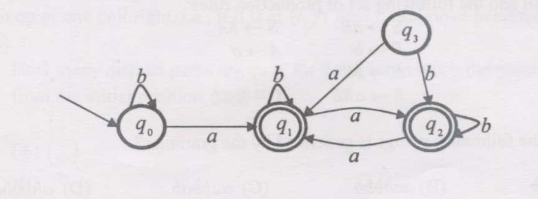
\includegraphics[width=0.5\linewidth]{figs/fig4.png}
    \caption{   }
    \label{fig4}
\end{figure}

\item The language accepted by this automaton is given by the regular expression
\begin{enumerate}
\begin{multicols}{4}
    \item $b^*ab^*ab^*ab^*$ 
    \item $(a+b)^*$ 
    \item $b^*a(a+b)^*$ 
    \item $b^*ab^*ab^*$
    \end{multicols}
\end{enumerate}
\hfill \textbf{(GATE EE 2025)}
\item The minimum state automaton equivalent to the above FSA has the following number of states:
\begin{enumerate}
\begin{multicols}{4}
    \item 1
    \item 2
    \item 3
    \item 4
    \end{multicols}
\end{enumerate}
\hfill \textbf{(GATE EE 2025)}
\newline
\textbf{Linked Answer Questions: Q.76 to Q.80 carry two marks each}
\newline
Suppose the letters a,b,c,d,e,f have probabilities $\frac{1}{2},\frac{1}{4},\frac{1}{8},\frac{1}{16},\frac{1}{32},\frac{1}{32}$ respeectively 


\item What is the following is the huffman code for the letters a,b,c,d,e,f?
\begin{enumerate}
    \item 0,10,110,1110,11110,11111
    \item 11,10,011,010,001,000
    \item 11,10,01,001,0001,0000
    \item 110,100,010,000,001,111
\end{enumerate}
\hfill \textbf{(GATE EE 2025)}
\item What is the average length of the correct answer to Q.76
\begin{enumerate}
\begin{multicols}{4}
    \item 3
    \item 2.1875
    \item  2.25
    \item 1.9375
    \end{multicols}
\end{enumerate}
 \hfill \textbf{(GATE EE 2025)}

\textbf{Statement for Linked Answer Questions 78 \& 79:}  

Consider the CFG with $\{S, A, B\}$ as the non-terminal alphabet, $\{a, b\}$ as the terminal alphabet, $S$ as the start symbol and the following set of production rules:
\[
\begin{aligned}
S &\to aB \quad &S &\to bA \\
B &\to bB \quad &A &\to a \\
B &\to bS \quad &A &\to aS \\
B &\to aBB \quad &A &\to bAA
\end{aligned}
\]




    
    \item Which of the following strings is generated by the grammar?
    \begin{enumerate}
    \begin{multicols}{4}
        
   
        \item aaabb
        \item aabbbb
        \item aabbab
        \item abbbba
         \end{multicols}
    \end{enumerate}
\hfill \textbf{(GATE EE 2025)}
    \item For the correct answer to Q.78, how many derivation trees are there?
    \begin{enumerate}
    \begin{multicols}{4}
        
    
        \item 1
        \item 2
        \item 3
        \item 4
        \end{multicols}
    \end{enumerate}

\hfill \textbf{(GATE EE 2025)}
\newline
\textbf{Statement for Linked Answer Questions 80 \& 81:}  

Consider a machine having an associated real memory size of $2^{16}$ bytes. Assume that a direct mapped data cache consisting of 32 lines of 64 bytes each is used in the system. A $50 \times 50$ two-dimensional array of bytes is stored in the main memory starting from memory location 1100H. Assume that the data cache is initially empty. The complete array is accessed twice. Assume that the contents of the data cache do not change in between the two accesses.


    
    \item How many data cache misses will occur in total?
    \begin{enumerate}
    \begin{multicols}{4}
        
   
        \item 48
        \item 50
        \item 56
        \item 59
         \end{multicols}
    \end{enumerate}
\hfill \textbf{(GATE EE 2025)}
    \item Which of the following lines of the data cache will be replaced by new blocks in accessing the array for the second time?
    \begin{enumerate}
    \begin{multicols}{2}
        
    
        \item line 4 to line 11
        \item line 4 to line 12
        \item line 0 to line 7
        \item line 0 to line 8
        \end{multicols}
    \end{enumerate}

\hfill \textbf{(GATE EE 2025)}
\newline
\textbf{Statement for Linked Answer Questions 82 \& 83:}  

A process has been allocated 3 page frames. Assume that none of the pages of the process are available in the memory initially. The process makes the following sequence of page references (reference string):  

$\textbf{1, 2, 1, 3, 7, 4, 5, 6, 3, 1}$



    
    \item If optimal page replacement policy is used, how many page faults occur for the above reference string?
    \begin{enumerate}
    \begin{multicols}{4}
        
    
        \item 7
        \item 8
        \item 9
        \item 10
        \end{multicols}
    \end{enumerate}
\hfill \textbf{(GATE EE 2025)}
    \item Least Recently Used (LRU) page replacement policy is a practical approximation to optimal page replacement. For the above reference string, how many more page faults may occur with LRU than with the optimal page replacement policy?
    \begin{enumerate}
    \begin{multicols}{4}
        
    
        \item 0
        \item 1
        \item 2
        \item 3
        \end{multicols}
    \end{enumerate}
 \hfill \textbf{(GATE EE 2025)}

\textbf{Statement for Linked Answer Questions 84 \& 85:}  

Suppose that a robot is placed on the Cartesian plane. At each step it is allowed to move either one unit up or one unit right, i.e., if it is at $(i,j)$ then it can move to either $(i+1,j)$ or $(i,j+1)$.


    
    \item How many distinct paths are there for the robot to reach the point $(10,10)$ starting from the initial position $(0,0)$?
    \begin{enumerate}
        \item $\binom{20}{10}$
        \item $2^{20}$
        \item $2^{10}$
        \item None of the above
    \end{enumerate}
\hfill \textbf{(GATE EE 2025)}
    \item Suppose that the robot is not allowed to traverse the line segment from $(4,4)$ to $(5,4)$. With this constraint, how many distinct paths are there for the robot to reach $(10,10)$ starting from $(0,0)$?
    \begin{enumerate}
        \item $2^{9}$
        \item $2^{8}$
        \item $2^{7}$
        \item None of the above
    \end{enumerate}
\hfill \textbf{(GATE EE 2025)}
\end{enumerate}
\end{document}



